\documentclass{article}

\usepackage[margin=1in]{geometry}
\usepackage{graphicx}

\begin{document}
\begin{titlepage}
	\clearpage\thispagestyle{empty}
	\centering
	\vspace{1cm}
		
	\rule{\linewidth}{1mm} \\[0.5cm]
	{ \Large \bfseries ISyE 6740 - Fall 2023\\[0.2cm]
		Project Proposal}\\[0.5cm]
	\rule{\linewidth}{1mm} \\[1cm]
 
		\begin{tabular}{l p{5cm}}
		\textbf{Team Member Names:} David Nguyen, Jorge Banegas, Thomas Algenio &  \\[10pt]
		\textbf{Project Title:} Decomposing and Classifying Real and Photoshopped Face Images &  \\[10pt]
		\end{tabular} 

        \begin{itemize}
            \item[] \textbf{Problem Statement}
        
            With the growing popularity of AI, countless positive contributions have been made to solve the world's toughest challenges. Along with these vast contributions to science and technology, there are also growing pain points when individual users leverage AI. In this research paper, we'll discuss the growing concerns within the computer vision category of AI. Although there are benefits of wanting to use AI to manipulate images (sharpening historical photos, facial recognition for identity verification, etc.), there are also reasons to use image manipulation techniques maliciously. A modern-day problem that has recently started becoming increasingly popular is the ability to create fake images of individuals that seem virtually realistic. This could lead to many adverse and undesirable effects for an individual. 
            
            Facial recognition has emerged as a pivotal technology in various sectors, from security and surveillance to personalized user experiences in digital platforms. However, with the proliferation of sophisticated image manipulation tools and generative models, the challenge of distinguishing genuine faces from artificially generated or manipulated ones has become paramount. Ensuring the accuracy and reliability of facial recognition systems in the face of these challenges is crucial. This paper aims to understand better the complexities of classifying these image types and evaluate techniques that will lead to reasonable classification rates. 
            
            \item[] \textbf{Data Source}

\begin{figure}[H]
\caption{Easy Level Fake Images}
\centering
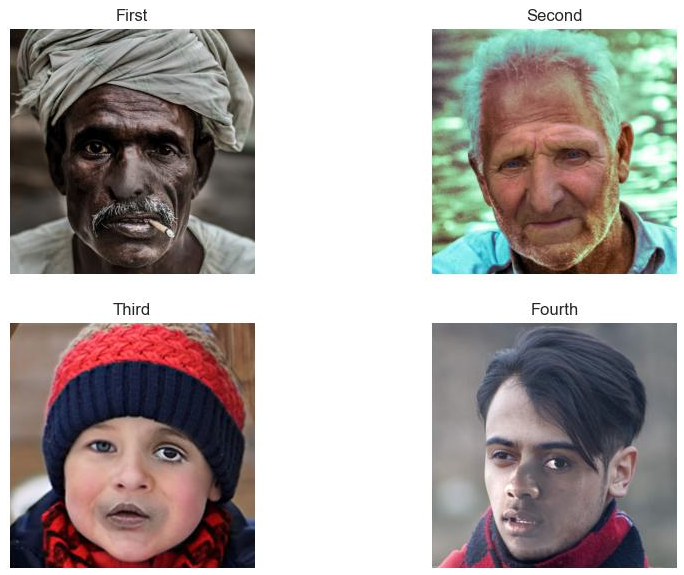
\includegraphics[width = 0.325\textwidth]{4_img_easy.png}
\caption{Medium Level Fake Images}
\centering
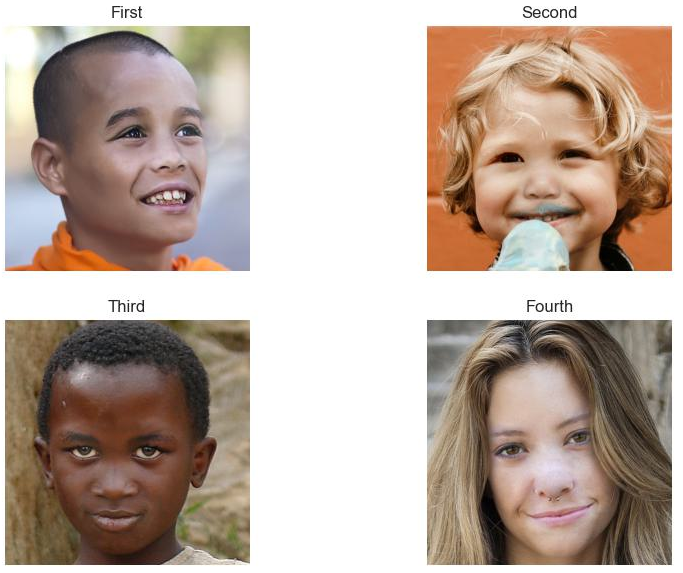
\includegraphics[width = 0.325\textwidth]{4_img_med.png}
\caption{Hard Level Fake Images}
\centering
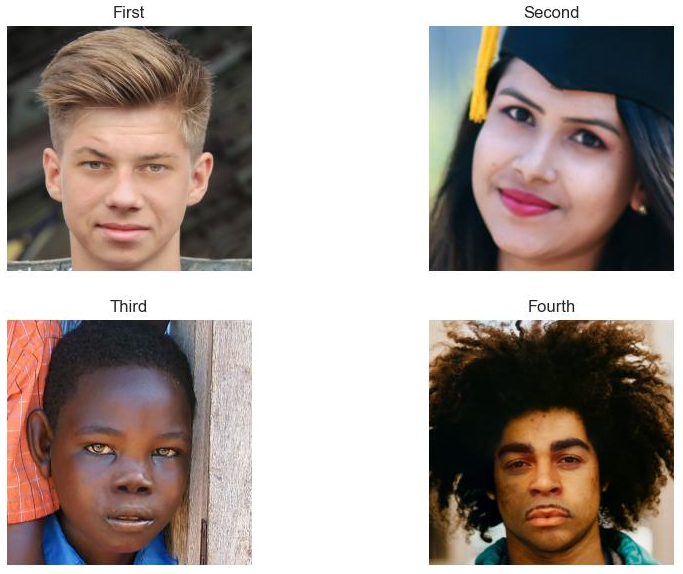
\includegraphics[width = 0.325\textwidth]{4_img_hard.png}
\caption{Real Images}
\centering
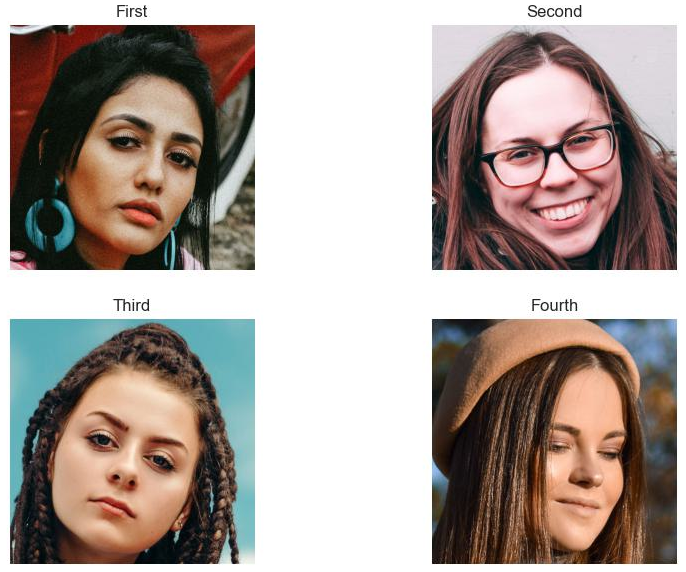
\includegraphics[width = 0.325\textwidth]{4_img_real.png}
\end{figure}

            Seonghyeon Nam, Seoung Wug Oh, Jae Yeon Kang, Chang Ha Shin, Younghyun Jo, Young Hwi Kim, Kyungmin Kim, Minho Shim, Sungho Lee, Yunji Kim, Suho Han, Gunhee Nam, Dasol Lee, Subin Jeon, In Cho, Woongoh Cho, Sejong Yang, Dongyoung Kim, Hyolim Kang, Sukjun Hwang, and Seon Joo Kim. (2019, January). Real and Fake Face Detection, Version 1. Retrieved [2023, September 19] from https://www.kaggle.com/datasets/ciplab/real-and-fake-face-detection.

            Our data is balanced based on the target value having close to a 1:1 ratio. The actual class label has a proportion of 52.96\% in total data points, while the fake class label has a proportion of 47.04\% in total data points. This early insight would indicate there is less of a need to use techniques to balance the targets within the data set, e.g., having to run K-Fold CV, SMOTE, etc...

\begin{center}
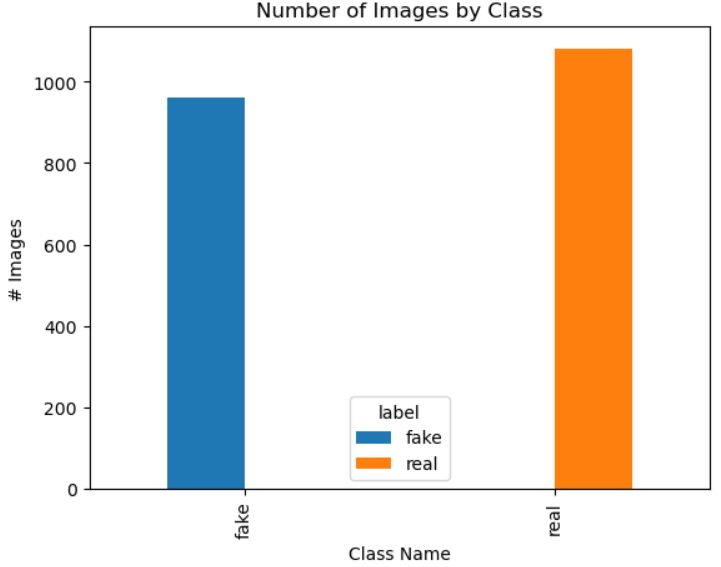
\includegraphics[width = 0.375\textwidth]{balance_histogram.png}
\end{center}

% 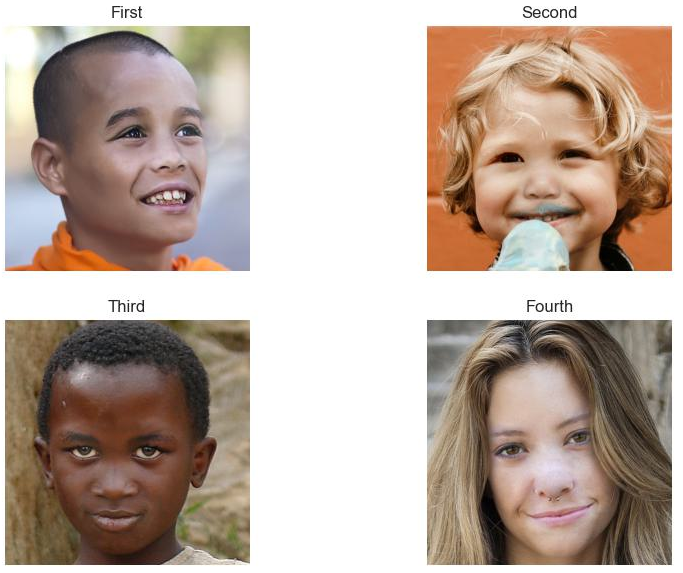
\includegraphics[width = 0.4\textwidth]{4_img_med.png}
% \end{center}

\newpage

            \item[] \textbf{Methodology}


            Due to the complexity of solving real-world problems, there is no "one-size-fits-all" approach. That being said, a mix of techniques will be combined to develop a more robust solution for classifying real and fake face images. One thing we will need to take into consideration is the varying dimensionality of each image. A conversion to a multi-dimensional matrix must be considered when dealing with any photos for computing. It's also vital that matrix sizes need to be consistent across images. Thus, the first step will transform the inputted image into a 1-D array.

\begin{center}
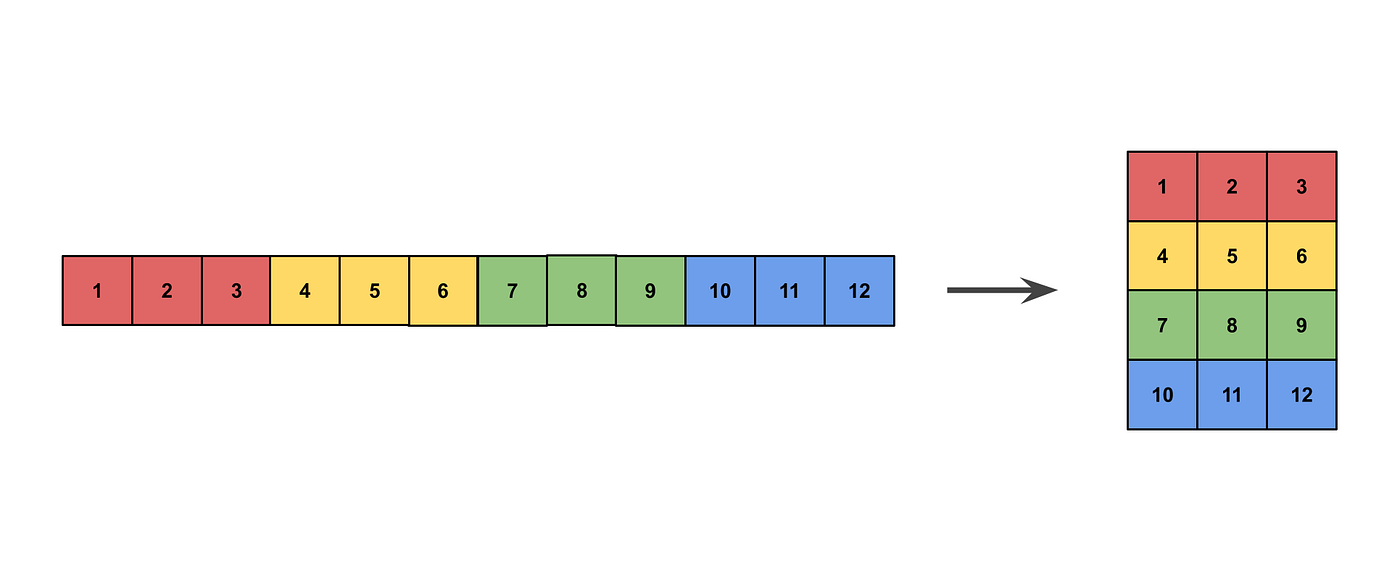
\includegraphics[width = 0.7\textwidth]{array.png}
\end{center}

    After the data transformation step, we can introduce different methodologies we want to implement. We will also be grouping our analytics models into a training and testing set to reduce model bias. Depending on the performance of the classification problems, we may need to increase the complexity of our solutions. We will begin our classification task with relatively more straightforward methodologies for classifying real and fake images. If our resulting accuracies are inadequate, we will increase our solutions' complexity and move on to the following method.

    \textbf{Method 1: PCA and ISOMAP 2-D Dimensionality Reduction and Unsupervised Clustering}

    We will test different dimensionality reduction algorithms and plot the images on a 2-D subspace. This will allow us to visualize similar pictures on a two-dimensional plot in which we can use a clustering algorithm to find similar shared features for real/fake photos and ignore image labels. To assess model accuracy, we can calculate the purity of each cluster by obtaining the number of images of real or fake photos out of all data points in each cluster set. We will treat this method as an unsupervised learning method to understand how the different image types are clustered. Ideally, fake images will be clustered similarly to each other, as well as authentic images.

\begin{center}
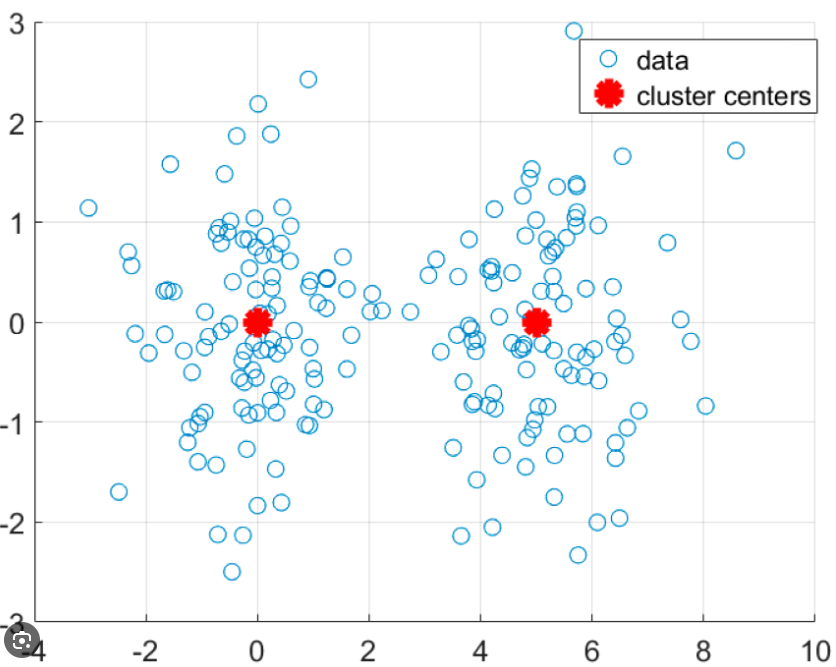
\includegraphics[width = 0.5\textwidth]{clustering.png}
\end{center}


\newpage


    \textbf{Method 2: PCA and ISOMAP 2-D Dimensionality Reduction and Labeled Classification}

    We will test different dimensionality reduction algorithms and plot the images on a 2-D subspace. This will allow us to visualize similar pictures on a two-dimensional plot. Instead of a clustering algorithm, we would leverage a classification model because we have a labeled set of real and fake images. Some potential classification models that could be used to generate predictions could be logistic regression, support vector machines, naive bayes, and K-Neighbors model. We can calculate the most notable binary classification metrics to assess model accuracy. We will treat this method as supervised learning to understand if the images can be mathematically separated into different groupings. Ideally, there will be a clear delineation between real and fake face image groups.

\begin{center}
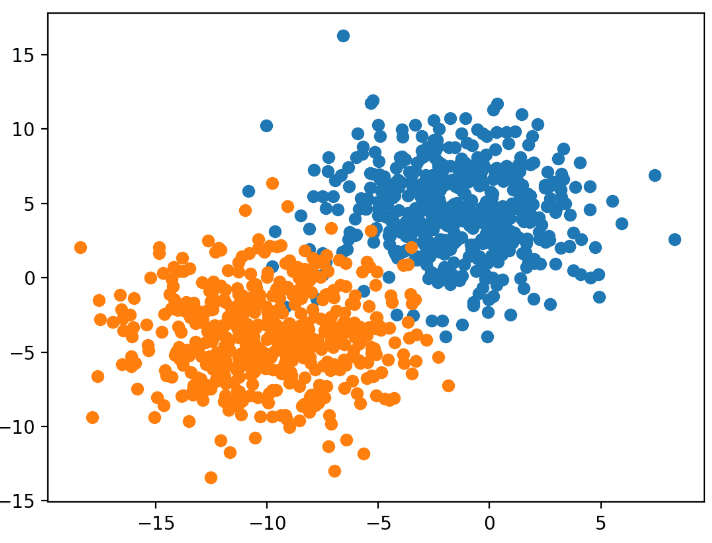
\includegraphics[width = 0.7\textwidth]{classification.png}
\end{center}

    \textbf{Method 3: Using Convolutional Neural Networks (CNN) for Classification on Labeled Data}

    Convolutional Neural Networks are deep learning models that automatically learn and adapt spatial hierarchies of features from images. They have been proven effective for not only classification tasks but image classification tasks as well.
     
    We will train a CNN on our vectorized data to distinguish between real and fake faces. The CNN will learn to recognize subtle patterns and inconsistencies in fake or manipulated images based on a training and validation set.

    We'll start with convolutional layers, each followed by a ReLU activation function and a max-pooling layer to reduce the spatial dimensions. This sequence helps the network to identify the local patterns and significant features of an image, such as focal points, edges, textures, and colors. As the depth of the network increases, these local features combine to form more global features, such as eyes, nose, and mouth. Finally, several fully connected layers will classify the image based on the recognized features.

    Given the possibility of over fitting due to limited data, there's a possibility of using image transformation and data augmentation techniques to increase the size of our training data set artificially. Randomly cropping, rotating, and horizontally flipping can help the model generalize better to new data.

    Given the complex nature of the problem and potential limited data set size, we may leverage pre-trained models like VGG16, ResNet, or Inception. Using these models, which have been trained on large data sets, could be an option to look into and fine-tune the top layers to work specifically to our use case.

    \textbf{Method 4 (Optional): PCA for Reducing Face on Lower Dimensional Space (Eigenfaces) and running Classification}

    Eigenfaces involves representing facial images in a lower-dimensional space using PCA. By projecting facial images onto a set of orthogonal vectors (Eigenfaces), we can capture the most significant features of the facial images. We will use Eigenfaces for the primary task of face recognition. We can identify the closest match by comparing the PCA weights of a new face with those in our database.

    If the dataset consists of images from different individuals, Eigenfaces becomes less ideal for distinguishing real from fake images. Eigenfaces works best when there are multiple images of the same person under different conditions, as it primarily captures the variance between different images of the same person. The primary goal of Eigenfaces is to reduce the high dimensionality of the face images into a more manageable space, capturing the significant features (or variance) of those faces. For a dataset of different people, each potentially with only one image representation, using Eigenfaces to differentiate between real and fake images can be challenging, as it might not adequately capture the correct type of variance.

    Instead of relying on PCA, we can leverage the power of pre-trained deep-learning models to extract robust features from the images, which can be used for classification.

    We can use pre-trained models like VGG16, ResNet, or Inception, which have been trained on vast datasets like ImageNet. Passing our images through these models and extracting features from one of the last layers (before classification layers), we get a rich representation of our images, capturing complex patterns.

Dimensionality Reduction: Even after using deep models for feature extraction, the feature vector can be high-dimensional. Techniques such as PCA, ISOMAP, t-SNE can be applied to these deep features for visualization or further analysis.

    Once we have our feature vectors, we can train a classifier, like a Logistic Regression model, Support Vector Machine (SVM), or a Random Forest classifier, to distinguish between real and fake images based on these features. These classifiers work well with high-dimensional data and can provide interpretability.

    

    

            \item[] \textbf{Evaluation and Final Results}

            As an outcome of this project, we would like to have developed a robust facial recognition system that not only identifies individuals based on facial features but also discerns real faces from fake or manipulated ones, ensuring the authenticity of the recognized faces. After the validation of our results, there will be a comprehensive report detailing the performance metrics of the classification system, including accuracy, precision, recall, and F1-score.

            One of the challenges that we could possibly face is the increasing sophistication of generative models, which can produce highly realistic fake images. We must also ensure that our systems align with privacy and ethical concerns associated with facial recognition technology and subject security. Diverse data sets could be challenging to work with due to needing a large enough sample size across demographics, including general lighting conditions and head orientations.

        \end{itemize}

	\pagebreak

\end{titlepage}


\end{document}
